\section{Introduction}
\label{sec:intro}

\begin{figure}[]
    \centering
    \vspace{-0.5cm}
    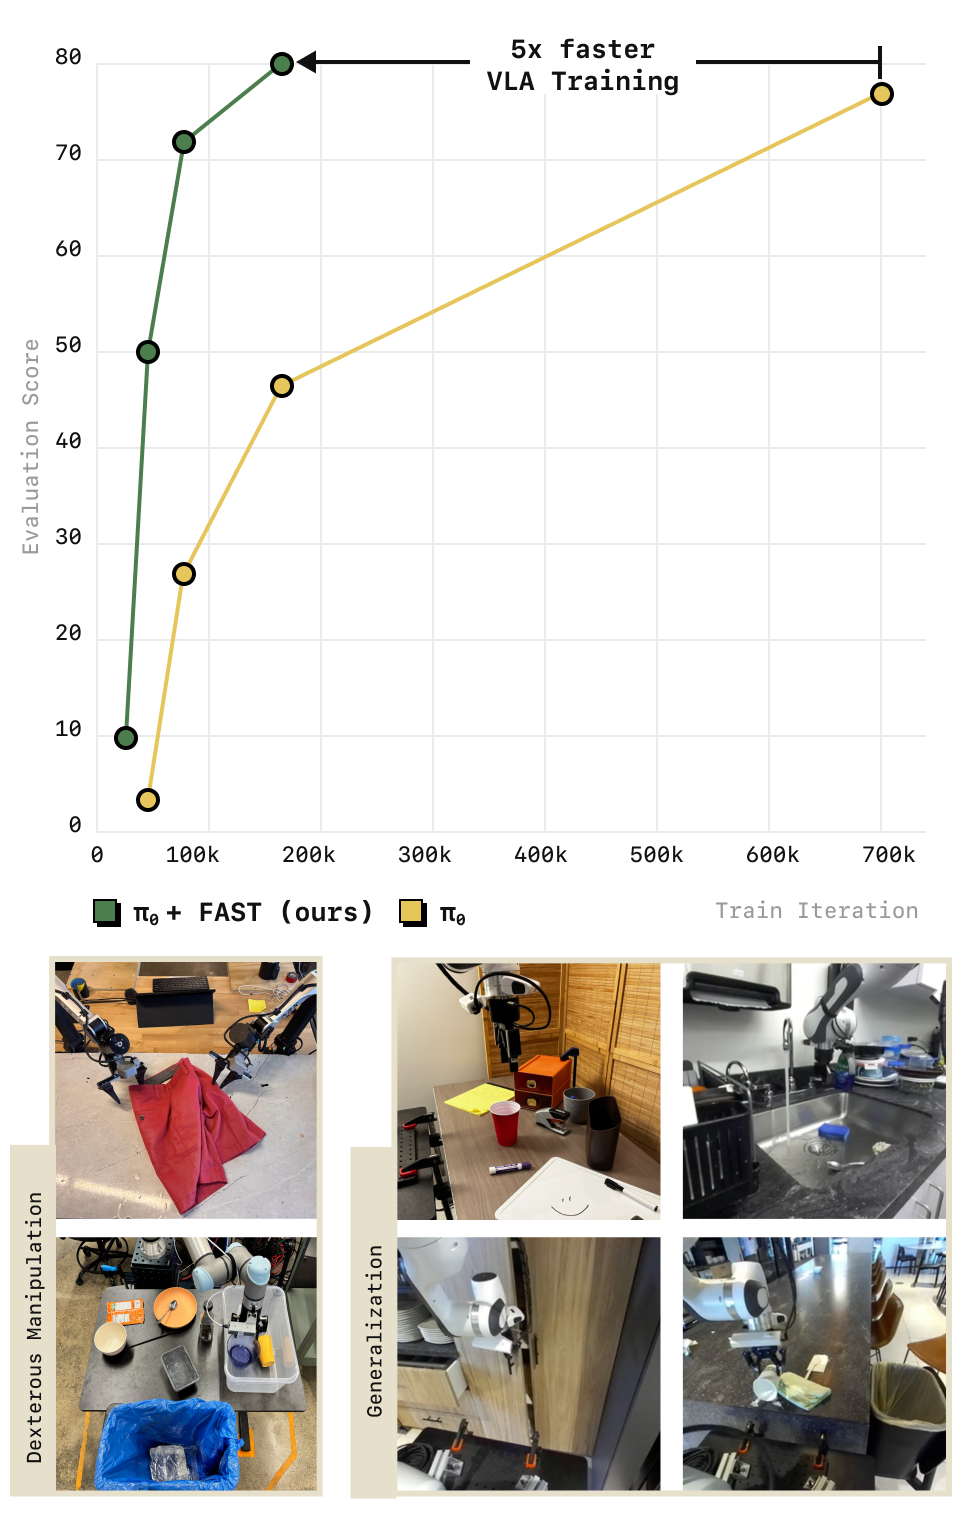
\includegraphics[width=\linewidth]{figures/convergence_2.jpg}
    \caption{We propose \ModelAcronym, a simple yet effective approach for tokenization of robot action trajectories via time-series compression. \ModelAcronym{} enables training of autoregressive VLAs that solve complex dexterous manipulation tasks and generalize broadly to new scenes. We use it to train \GeneralistModelAcronym{}, a generalist robot policy that matches the performance of the state-of-the-art $\pi_0$ diffusion VLA on dexterous and long-horizon manipulation tasks, while training 5x faster (\textbf{top}).
    }
    \label{fig:convergence}
    \vspace{-1.5em}
\end{figure}

Large, high-capacity Transformer models can be tremendously effective for capturing complex and generalizable robotic behaviors both from scratch~\citep{rt12022arxiv,zhao2023learning,octo_2023,bharadhwaj2023roboagent,Doshi24-crossformer, wangscaling} and using models pre-trained for next-token prediction on Internet-scale image-text corpora~\citep{rt22023arxiv,kim2024openvla,wen2024tinyvlafastdataefficientvisionlanguageaction,black2024pi_0,ye2024latent}.
However, these models require choosing a tokenization of the continuous action signal, which determines how the discrete symbols predicted by the model map to continuous robot actions~\citep{yan2024elastictok,jang2024efficient,lee2024behavior,chen2022beats}. It is widely known that a good choice of tokenization can be critical to the performance of sequence models~\citep{radford2019language, sennrich2015neural}. Prior robotic policies of this sort typically use na\"{i}ve tokenization strategies based on a per-dimension, per-timestep binning scheme~\citep{brohan2022rt,rt22023arxiv,kim2024openvla}.
We find that such methods perform poorly when learning dexterous skills with high-frequency control (see \cref{fig:teaser}, right). We observe that correlations between time steps are a major challenge for na\"{i}ve tokenization strategies when predicting sequences of future actions, i.e., action ``chunks'', as is common for high-frequency control. Highly correlated action tokens \emph{diminish} the effectiveness of the next token prediction objective used in autoregressive VLAs. Intuitively, in such cases low token prediction loss can often be achieved with mappings as trivial as simply copying the most recent action token, leaving models in poor local optima.


In this work, we propose a new tokenization strategy from first principles. Our key insight is that robot action signals need to be \emph{compressed} before training, to reduce correlation between consecutive tokens. We take inspiration from compression-based tokenization strategies, such as the byte-pair encoding method commonly used by language models~\citep{gage1994new, sennrich2015neural}. However, since robotic actions are continuous, the corresponding compression strategy should be chosen accordingly. We therefore base our method off of the discrete cosine transform~(DCT) encoding, which is widely used for compressing continuous signals such as images (e.g., JPEG compression).
We find that the resulting tokenization approach, \ModelAcronymLong, enables us to train autoregressive VLA policies via simple next token prediction (see \cref{fig:teaser}, left) for highly dexterous and high-frequency tasks where standard discretization methods fail entirely. 
Additionally, \ModelAcronym{} for the first time enables efficient VLA training on the recently introduced DROID dataset~\citep{khazatsky2024droid}, a large-scale multitask ``in-the-wild'' robot manipulation dataset. The resulting policy is the first language-conditioned generalist manipulation policy that can be successfully evaluated \emph{zero-shot} in unseen environments, simply by prompting it in natural language.

\begin{figure}[t]
    \centering
    
\includegraphics[width=\linewidth]{figures/teaser.pdf}
    \caption{\textbf{Left}: \ModelAcronym{} tokenization enables training of autoregressive Transformers for dexterous robot control via simple next token prediction. \textbf{Right}: \ModelAcronym{} outperforms popular binning tokenization schemes, e.g., used in OpenVLA~\citep{kim2024openvla}, particularly for high-frequency robot data.
    }
    \label{fig:teaser}
\end{figure}

Based on \ModelAcronym{}, we develop \ModelUniversalAcronym, a \textbf{\underline{universal} robot action tokenizer}, trained on 1M real robot action trajectories that cover a large diversity of robot embodiments, action spaces and control frequencies. We demonstrate that the \ModelUniversalAcronym~tokenizer effectively tokenizes a wide range of robot action sequences, from single-arm to bi-manual and mobile robots, and is a good off-the-shelf tokenizer for training autoregressive VLA models. When integrated with the $\pi_0$ VLA, FAST-based autoregressive VLAs scale to training on 10k hours of robot data and achieve performance comparable to diffusion-based VLAs across a variety of tasks, while reducing training time by up to 5x (see \cref{fig:convergence}).








